\section{Exercise 9}
\subsection{}
To solve these questions we have defined a few functions which represent the values of the 2 given options. Go left and don't cross the bridge and cross the bridge. We have chosen X axis to represent the discount and Y axis to represent value / score of the given function / option. \\ \smallskip
\begin{itemize}
  \item Agent will never cross the bridge is only discount is changed. See \Fgcite{fig:e91}. The green lines is always on top.
  \item AgentAgent is able to cross the bridge when discount is 0.9 and noise is lower than 0.01695. This is because the the value functions cross below discount of 0.9 around this value. \Fgcite{fig:e92}
\end{itemize}

\begin{figure}[H]
\caption{}
\centering
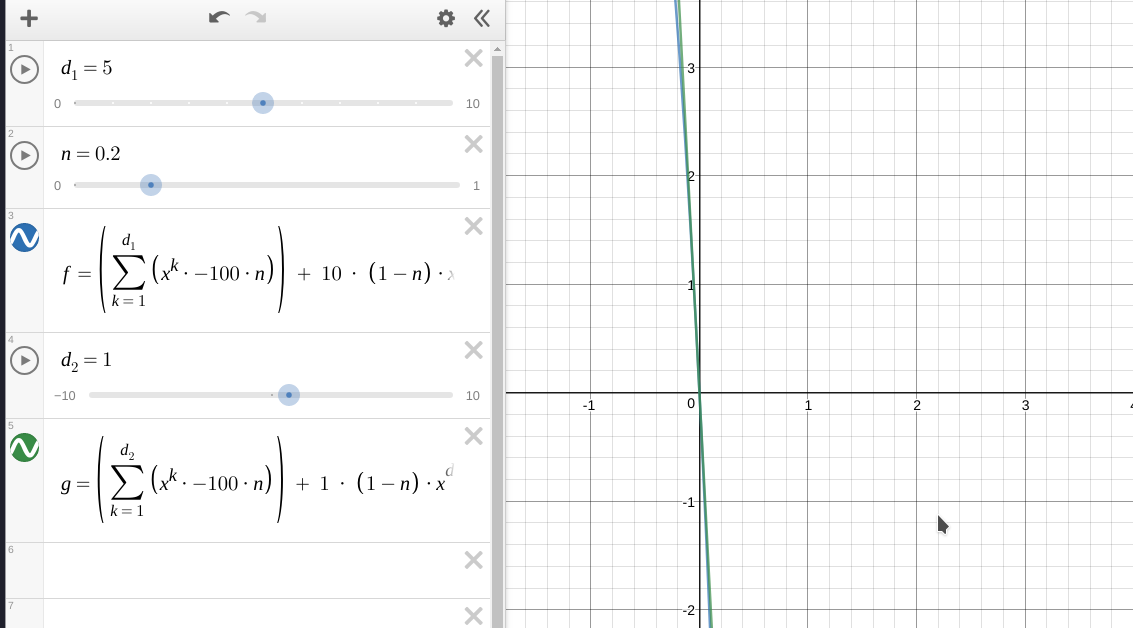
\includegraphics[width=12cm]{plot_9_1}
Blue = Cross the bridge values \\ 
Red = Take reward on the left \\
Noise = 0.2
\label{fig:e91}
\end{figure}

\begin{figure}[H]
\caption{}
\centering
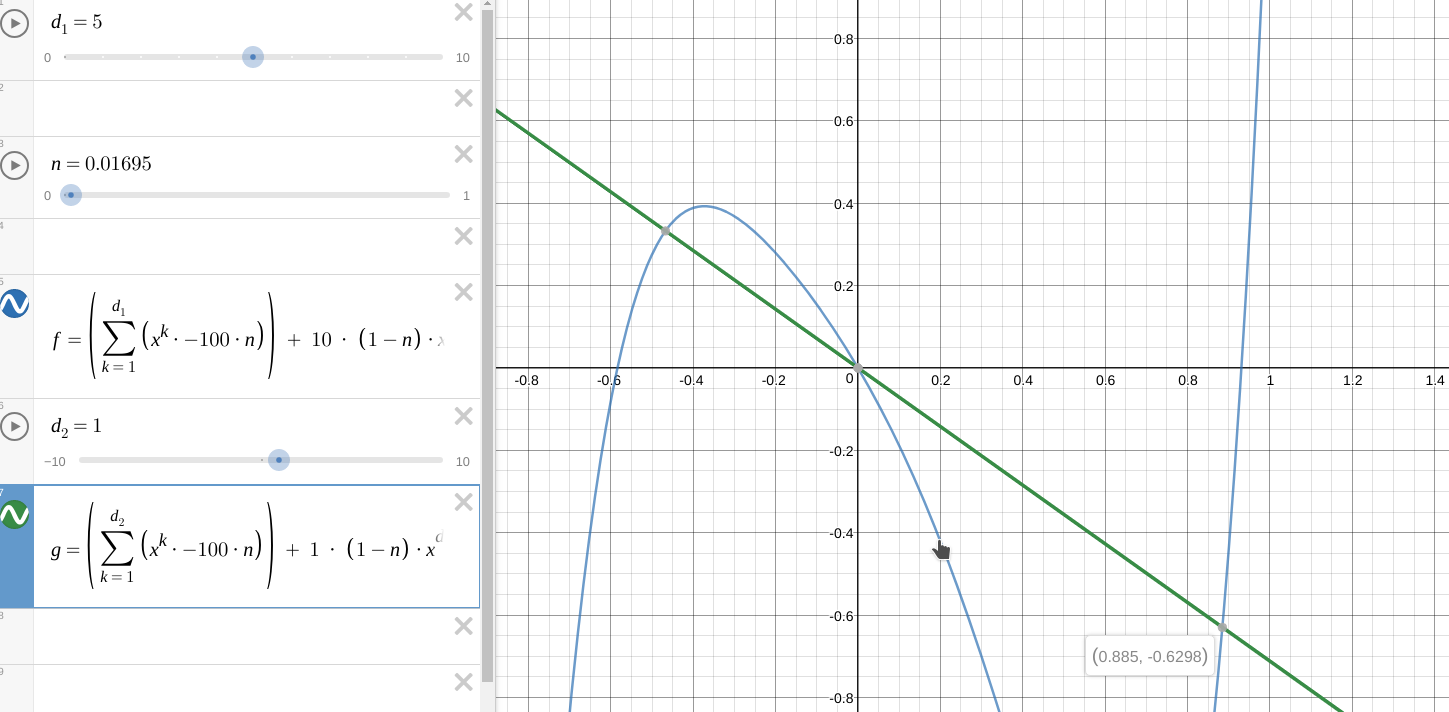
\includegraphics[width=12cm]{plot_9_2}
Blue = Cross the bridge values \\ 
Red = Take reward on the left \\
Noise = 0.01695
\label{fig:e92}
\end{figure}

\subsection{}
We have changed the noise parameter, since it is not possible to do this by only changing the discount. See explanation above. We have chosen 0.01695 as noise value since it lies right on the border of possible noise values which allow agent to cross the bridge. Values lower than this one will give same results and values above* won't.